% This file was created by matlab2tikz.
%
%The latest updates can be retrieved from
%  http://www.mathworks.com/matlabcentral/fileexchange/22022-matlab2tikz-matlab2tikz
%where you can also make suggestions and rate matlab2tikz.
%
\definecolor{mycolor1}{rgb}{0.00000,0.44700,0.74100}%
\definecolor{mycolor2}{rgb}{0.85000,0.32500,0.09800}%
\definecolor{mycolor3}{rgb}{0.92900,0.69400,0.12500}%
%
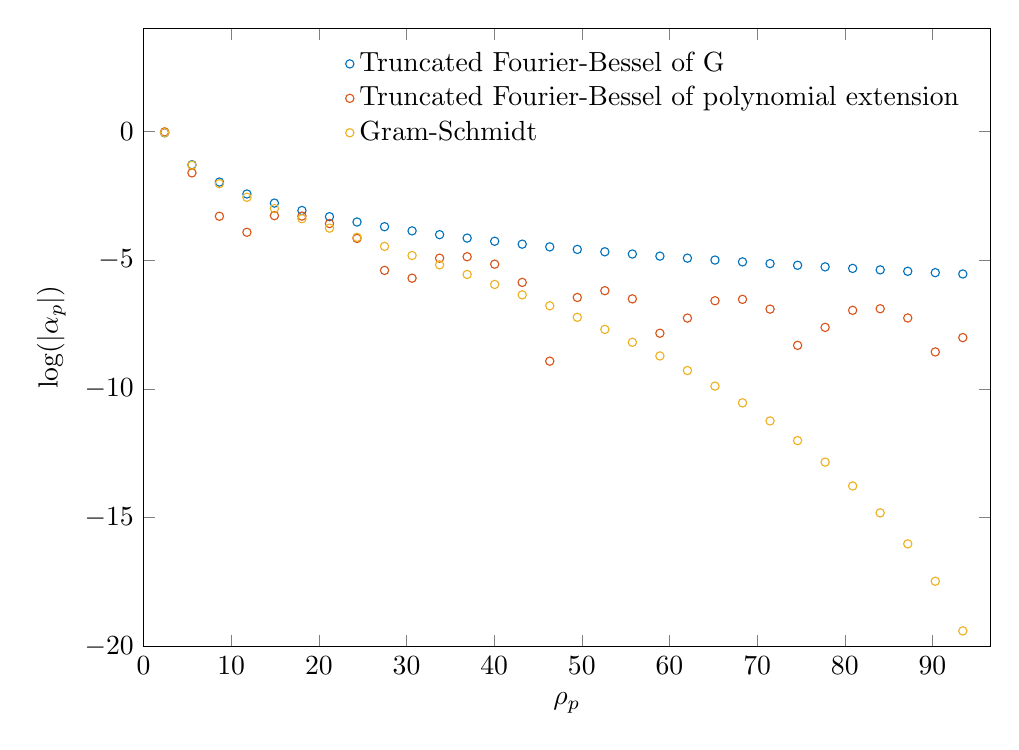
\begin{tikzpicture}

\begin{axis}[%
width=4.234in,
height=3.091in,
at={(1.045in,0.956in)},
scale only axis,
xmin=0,
xmax=96.6053053182372,
xlabel={$\rho_p$},
ymin=-20,
ymax=4,
ylabel={$\log(|\alpha_p|)$},
axis background/.style={fill=white},
legend style={legend cell align=left,align=left,fill=none,draw=none}
]
\addplot[only marks,mark=o,mark options={},mark size=1.5000pt,color=mycolor1] plot table[row sep=crcr]{%
2.40482555762315	-0.0595560186878546\\
5.52007810274485	-1.29892142374055\\
8.65372791289424	-1.97218007969845\\
11.7915344388313	-2.43589439418346\\
14.9309037381854	-2.78980664404281\\
18.0710639678808	-3.07603559603896\\
21.211626861317	-3.31634047814016\\
24.3524495360216	-3.52343229092601\\
27.4934725322526	-3.70538296001701\\
30.6345898998327	-3.86763910444304\\
33.7758159545786	-4.01404963200899\\
36.917084913022	-4.14743519676087\\
40.0584232777753	-4.26992462969729\\
43.1997802848901	-4.38316414330123\\
46.3411872641951	-4.48845299808829\\
49.4825998634098	-4.58683461918007\\
52.6240518346981	-4.67915963917424\\
55.7655017400859	-4.76613064610321\\
58.9069848173393	-4.84833465886013\\
62.0484609504762	-4.92626715959704\\
65.1899664364413	-5.00035018724746\\
68.3314616987713	-5.07094617054835\\
71.472983868065	-5.13836865040029\\
74.6144935024883	-5.20289069491361\\
77.7560284312404	-5.26475157841005\\
80.8975491323772	-5.32416213716151\\
84.0390940409322	-5.38130910449939\\
87.1806234414138	-5.4363586501388\\
90.3221763051478	-5.48945929281651\\
93.4637126646474	-5.54074431485235\\
};
\addlegendentry{Truncated Fourier-Bessel of G};

\addplot[only marks,mark=o,mark options={},mark size=1.5000pt,color=mycolor2] plot table[row sep=crcr]{%
2.40482555762315	-0.0231838178905557\\
5.52007810274485	-1.61535852964004\\
8.65372791289424	-3.2997785403795\\
11.7915344388313	-3.92163929254402\\
14.9309037381854	-3.27585161655716\\
18.0710639678808	-3.29180320065408\\
21.211626861317	-3.58350749665352\\
24.3524495360216	-4.16085366882024\\
27.4934725322526	-5.40187997600935\\
30.6345898998327	-5.70396506211945\\
33.7758159545786	-4.92756813027028\\
36.917084913022	-4.87066720372305\\
40.0584232777753	-5.16018044719195\\
43.1997802848901	-5.86791386494028\\
46.3411872641951	-8.92563252093615\\
49.4825998634098	-6.45271352136794\\
52.6240518346981	-6.18990871930147\\
55.7655017400859	-6.50606359148113\\
58.9069848173393	-7.84113308543085\\
62.0484609504762	-7.25341319951939\\
65.1899664364413	-6.5793678281535\\
68.3314616987713	-6.52570184397092\\
71.472983868065	-6.90534568022029\\
74.6144935024883	-8.31113534777972\\
77.7560284312404	-7.61375004073648\\
80.8975491323772	-6.95188808123909\\
84.0390940409322	-6.88949537982059\\
87.1806234414138	-7.24946050129589\\
90.3221763051478	-8.56759870375677\\
93.4637126646474	-8.01109815285378\\
};
\addlegendentry{Truncated Fourier-Bessel of polynomial extension};

\addplot[only marks,mark=o,mark options={},mark size=1.5000pt,color=mycolor3] plot table[row sep=crcr]{%
2.40482555762315	-0.052408399766762\\
5.52007810274485	-1.31665841112951\\
8.65372791289424	-2.03476760128999\\
11.7915344388313	-2.56344881184711\\
14.9309037381854	-3.00265144707083\\
18.0710639678808	-3.3947692499593\\
21.211626861317	-3.76190961569123\\
24.3524495360216	-4.11721108143688\\
27.4934725322526	-4.46926024598518\\
30.6345898998327	-4.82411531720457\\
33.7758159545786	-5.18634598224769\\
36.917084913022	-5.55961827025646\\
40.0584232777753	-5.94705037601962\\
43.1997802848901	-6.35144642065153\\
46.3411872641951	-6.77546347280186\\
49.4825998634098	-7.22174313111453\\
52.6240518346981	-7.69302747737406\\
55.7655017400859	-8.19227408853041\\
58.9069848173393	-8.72278354351784\\
62.0484609504762	-9.28835477543871\\
65.1899664364413	-9.89348928383497\\
68.3314616987713	-10.5436768090679\\
71.472983868065	-11.245817729079\\
74.6144935024883	-12.0088831109859\\
77.7560284312404	-12.8450115103249\\
80.8975491323772	-13.7714725961456\\
84.0390940409322	-14.8145417661211\\
87.1806234414138	-16.0182637778206\\
90.3221763051478	-17.4689726486279\\
93.4637126646474	-19.3975469826778\\
};
\addlegendentry{Gram-Schmidt};

\end{axis}
\end{tikzpicture}%